\documentclass[../kl11.tex]{subfiles}
\graphicspath{{\subfix{../images/}}}


\begin{document}

\section{Ziegler-Natta-Katalysatoren unter der Lupe}
In der Polymerindustrie spielen verschiedene Kettenwachstumsmechanismen eine Rolle. Es gibt radikalische, kationische oder anionische Kettenpolymerisation. Eine weitere Möglichkeit ist der koordinative Kettenwachstumsmechanismus. Ein Beispiel für eine Anwendung der koordinativen Polymerisation ist die Herstellung von Polypropylen aus Propen.

 \enumersteaufgabe{\operator{Gib} die Struktur von Polypropylen \operator{an} und \operator{bestimme}, wie viele Moleküle Propylen notwendig sind, um \SI{5}{\kg} Polypropylen zu erzeugen.}
 \solution{
 
\includegraphics[width=0.2\textwidth]{2024/Abbildungen/Ziegler-Natta/L_a.eps}
 $N_{\mathrm{Propen}}=N_\mathrm{A}\cdot n_{\mathrm{Propen}}=N_\mathrm{A}\cdot m/M_{\mathrm{Propen}} =7,155 \cdot 10^{25}$\\
 1 P. für richtige Strukturformel (kann auch äquivalente andere Schreibweise sein, z.B. Lewis-Formel etc.), 1 P. für richtiges Ergebnis\\
 insg. 2 P.
}{7cm}
 \enumaufgabe{\operator{Kreuze an}, welche der folgenden Punkte allgemein auf Katalysatoren zutreffen und welche nicht.}
 \begin{tabularx}{\textwidth}{|X|C{1.5cm}|C{1.5cm}|}\hline
     & wahr & falsch\\\hline
     Erhöht die Reaktionsgeschwindigkeit einer Reaktion & \solutiontext{\checkedbox}{\emptybox} & \emptybox \\\hline
     Ist eine Lewis-Säure & \emptybox	& \solutiontext{\checkedbox}{\emptybox} \\\hline
     Ist eine Lewis-Base	& \emptybox & \solutiontext{\checkedbox}{\emptybox} \\\hline
     Erniedrigt die Aktivierungsenergie einer Reaktion & \solutiontext{\checkedbox}{\emptybox} & \emptybox \\\hline
     Verschiebt das Gleichgewicht auf die Seite der Produkte & \emptybox & \solutiontext{\checkedbox}{\emptybox} \\\hline
     Verlangsamt Nebenreaktionen & \emptybox & \solutiontext{\checkedbox}{\emptybox} \\\hline
 \end{tabularx}
 \solutiontext{je 0,5 P. $\longrightarrow$ 3 P.
 }{}

 Um den Prozess der Polymerisation zu katalysieren, werden Übergangsmetallverbindungen verwendet. Meistens finden \textsc{Kaminsky}-Katalysatoren Anwendung. Diese leiten sich von den sogenannten Metallocenen ab. Metallocene sind metallorganische Verbindungen bestehend aus zwei Cyclopentadienylliganden und einem Metallzentralteilchen.
 Ein Beispiel für einen \textsc{Kaminsky}-Katalysator ist das Zirkonocendichlorid \textbf{Z}, welches durch einen Cokatalysator in die aktive Katalyseform \textbf{Z‘} überführt wird.
 \begin{figure}[H]
     \centering
     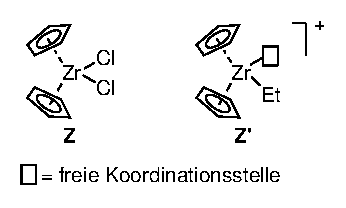
\includegraphics[width=0.6\linewidth]{2024/Abbildungen/Ziegler-Natta/ZZ.eps}
 \end{figure}
\newpage
 \enumaufgabe{\operator{Begründe} unter Betrachtung der Gesamtelektronenzahl des Zirkoniums, ob Zirkonocendichlorid \textbf{Z} oder die aktive Form \textbf{Z‘} stabiler und/oder reaktiver ist.}
 \solution{
 Gesamtelektronen für \textbf{Z}: $0 + 2\cdot6 + 2\cdot2 = 16$\\
 Gesamtelektronen für \textbf{Z’}: $0 + 2\cdot6 + 2 = 14$\\
 1,5 P. pro richtige Gesamtelektronenzahl\\
 \textbf{Z} ist stabiler, weil es näher an den 18 Elektronen ist, als \textbf{Z‘} (1 P.)\\
\textbf{Z‘} reagiert deshalb (unter Assoziation von Liganden) weiter (0,5 P.)\\
 insg. 4,5 P.
 }{5cm}
 Die aktive Form \textbf{Z‘} wird meist durch Reaktion von \textbf{Z} mit einem \textsc{Lewis}-sauren Alkylierungsmittel wie \ce{AlEt3} hergestellt. Dabei ist der erste Schritt eine Substitutionsreaktion. Danach zeigt sich die \textsc{Lewis}-Acidität der Aluminiumverbindung, was zu einer Chlorid-Übertragung führt.
 \enumaufgabe{\operator{Gib} die Teilreaktionsgleichungen für die Bildung von \textbf{Z‘} ausgehend von \textbf{Z} \operator{an}. \\\operator{Zeichne} dabei immer die Zirkoniumverbindung.}
 \solution{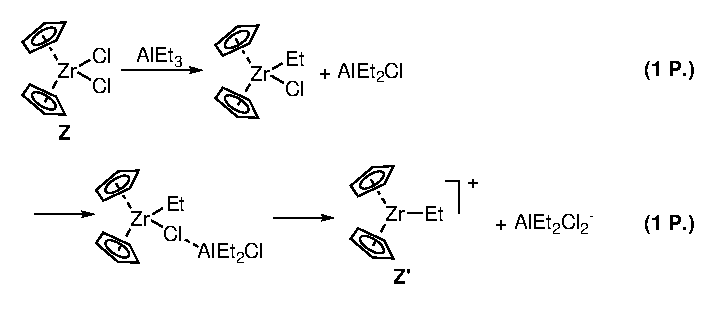
\includegraphics[width=1\textwidth]{2024/Abbildungen/Ziegler-Natta/L_d.eps}\\
 Reaktionsschritt 2 muss nicht in 2 Teilschritte aufgeteilt werden. Solange Eliminierung von \ce{AlEt2Cl2-} (bzw. \ce{AlEt3Cl-}) ersichtlich ist, gibt es den Punkt\\
 \ce{AlCl3} oder ähnliche Aluminiumspezien sind als Reagenz gleich zu bewerten wie \ce{AlEt2Cl} und \ce{AlEt2Cl2+}\\
 Jede Zirconiumspezies (3) jeweils 0,5 P.\\
 Insg. 3,5 P.}{14cm}
 \newpage
 Olefine weisen durch die Doppelbindungen elektronenreiche Bindungen auf. Diese können an leeren Koordinationsstellen von Übergangsmetallkomplexen über die $\pi$-Bindungen als Liganden binden.
 \enumaufgabe{\operator{Zeichne} die Struktur der Spezies \textbf{ZP}, die sich unmittelbar aus \textbf{Z‘} in der Gegenwart von Propen ergibt.}
 \solution{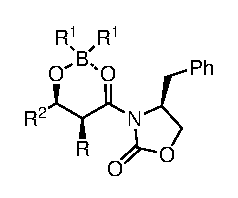
\includegraphics[width=0.3\textwidth]{2024/Abbildungen/Ziegler-Natta/L_e.eps} 1 P.}{5cm}
 \enumaufgabe{\operator{Zeichne} einen Mechanismus, wie aus \textbf{ZP} eine verlängerte Alkylkette entstehen kann.}
 \solution{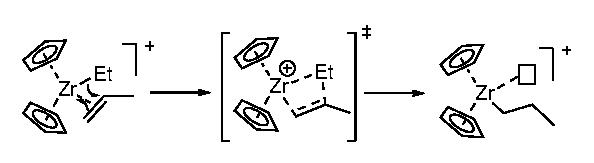
\includegraphics[width=0.9\textwidth]{2024/Abbildungen/Ziegler-Natta/L_f_alt.eps} \\
 1 P. für Elektronenschiebepfeile\\
 1 P. für korrektes Produkt (freie Koordinationsstelle nicht zwingend, da auch bei \textbf{Z'} nicht dargestellt)\\
 Übergangszustand 1 P.\\
 insg. 3 P.
 }{7cm}
 Eine Verbindung, die im Gesamtmechanismus der koordinativen Polymerisation auftritt, ist das Intermediat \textbf{I}. 
 \begin{figure}[H]
     \centering
     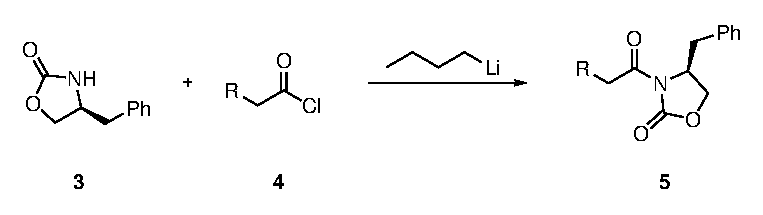
\includegraphics[width=0.35\linewidth]{2024/Abbildungen/Ziegler-Natta/2.eps}
 \end{figure}

 Dabei bindet ein Wasserstoffatom der Alkylkette zusätzlich an das Zentralmetall. Hierbei liegt eine agostische Wechselwirkung vor, bei der die Bindungselektronen des Wasserstoffs nicht wie typischerweise nur an den Kohlenstoff gebunden sind, sondern in Form einer Mehrzentrenbindung auch zwischen Metallzentrum und Wasserstoffatom delokalisiert vorliegen.
 \newpage
 \enumaufgabe{\operator{Erkläre}, aus welcher Eigenschaft des Zentralmetalls die besonderen Bindungsverhältnisse im Intermediat~\textbf{I} resultieren.}
 \solution{Aufgrund des Elektronenmangels (1 P.) von nur 14 VE sucht das Zentralteilchen mehr Elektronen durch Mehrzentrenbindung mit dem in $\beta$-Stellung benachbarten H-Atom.\\
 Andere Formulierungen ebenfalls korrekt (wichtig: ungesättigtes Zentralatom mit Elektronenmangel muss erwähnt werden)\\
 insg. 1\,P.
 }{3cm}
 Aus Intermediat~\textbf{I} lässt sich bereits eine mögliche Abbruchreaktion ableiten. Dabei entstehen eine neue Metallverbindung und die beendete Kette.
 \enumaufgabe{\operator{Gib} die Reaktionsprodukte der angesprochenen Abbruchreaktion \operator{an}.}
 \solution{
 
\includegraphics[width=0.35\linewidth]{2024/Abbildungen/Ziegler-Natta/L_h1.eps} oder
 
\includegraphics[width=0.25\linewidth]{2024/Abbildungen/Ziegler-Natta/L_h2.eps}\\
 1,5 P. wenn entweder dissoziert (links) oder noch assoziert (rechts) gezeichnet
 }{4cm}
 \enumaufgabe{\operator{Erkläre}, ob der Metallkatalysator im Zuge der Abbruchreaktion verbraucht wird oder nicht.} 
 \solution{Das resultierende Metallhydrid liegt immer noch in der katalytisch aktiven 14VE Form vor (1\,P.). \\
 Zudem kann in die Zr-H-Bindung wieder ein Olefin insertieren, womit eine neue Kette gestartet wird (1\,P.). Somit ist der Katalysator nicht verbraucht.\\
 insg. 2\,P.}{3cm}
 Die häufig dargestellte Wechselwirkung zwischen Doppelbindungen von Alkenen und dem Metallzentrum kann durch die Orbitalwechselwirkung des $\pi$- und des $\pi^\ast$-Molekülorbitals mit jeweils einem d-Orbital des Metallzentrums erklärt werden. Dabei treten zwei Arten von Bindungen auf. Bei der Bindung des besetzten $\pi$-Orbitals mit einem d-Orbital liegt die Elektronendichte auf der Bindungsachse zwischen Doppelbindung und Metallzentrum. Bei der Bindung des unbesetzten $\pi^\ast$-Orbitals mit einem d-Orbital liegt die Elektronendichte über und unter der Bindungsachse.
 \enumaufgabe{\operator{Benenne} die beiden Bindungsarten.\\Hinweis: Bei den Bindungen handelt es sich um $\sigma$-, $\pi$- und / oder $\delta$-Bindung}
 \solution{$\sigma$-Donor-Bindung und $\pi$-Akzeptor-Bindung\\
 jew. 1 P., wenn nur $\sigma$- oder $\pi$-Bindung dann jew. 0,5 P.; Hin- und Rückbindung sind als richtig zu werten\\
 Insg. 2 P.
 }{2cm}
 \newpage
 \enumaufgabe{\operator{Nenne} pro Bindungsart ein d-Orbital, das für die Bindungsbildung verantwortlich sein könnte, falls die Bindungsachse entlang der $z$-Achse orientiert ist.}
 \solution{für $\sigma$-Donor: $d_{z^2}$ 		1 P.\\
 für $\pi$-Akzeptor: $d_{xz}$ oder $d_{yz}$	1 P.\\
 Insg. 2 P.
 }{2cm}
 \enumaufgabe{\operator{Zeichne} die Wechselwirkungen der Orbitale in beiden Bindungen.}
 \solution{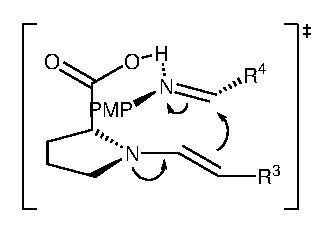
\includegraphics[width=0.2\textwidth]{2024/Abbildungen/Ziegler-Natta/L_k.eps}\\
 1\,P. für richtiges $\pi$-Orbital (auch richtig, wenn überlappendes $\pi$-Orbital statt beiden p-Orbitalen gezeichnet)
 1\,P. für richtiges $\pi$*-Orbital
 1\,P. für richtiges $d_z2$-Orbital
 1\,P. für richtiges $d_{xz}$ oder $d_{yz}$ – Orbital
 1\,P. pro richtige Überlappung/Vorzeichen (insgesamt 2\,P.)\\
 Insg. 6 P.
 }{8cm}
\solutiontext{$\sum$ 31,5 P.}{}
\end{document}